% This file was created with tikzplotlib v0.10.1.
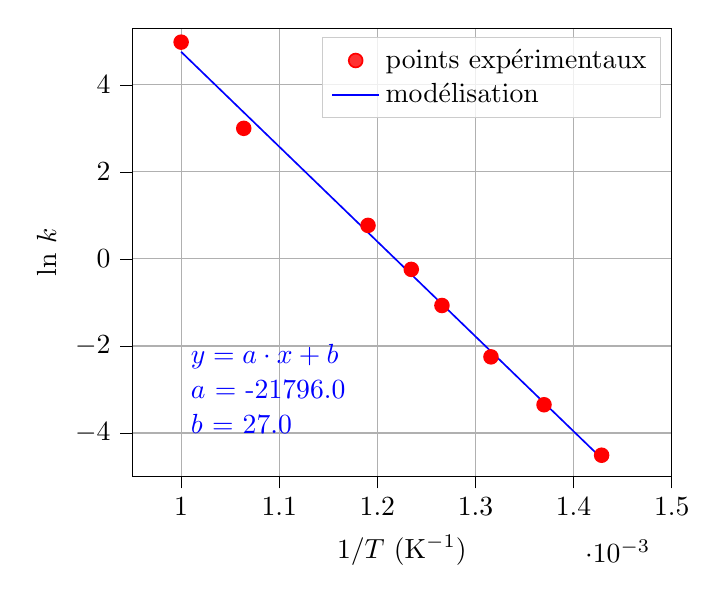
\begin{tikzpicture}

\definecolor{darkgray176}{RGB}{176,176,176}
\definecolor{lightgray204}{RGB}{204,204,204}

\begin{axis}[
legend cell align={left},
legend style={fill opacity=0.8, draw opacity=1, text opacity=1, draw=lightgray204},
tick align=outside,
tick pos=left,
x grid style={darkgray176},
xlabel={1/\(\displaystyle T\) (K\(\displaystyle ^{-1})\)},
xmajorgrids,
xmin=0.00095, xmax=0.0015,
xtick style={color=black},
y grid style={darkgray176},
ylabel={ln \(\displaystyle k\)},
ymajorgrids,
ymin=-5, ymax=5.3,
ytick style={color=black}
]
\addplot [semithick, red, mark=*, mark size=2.5, mark options={solid}, only marks]
table {%
0.00142857142857143 -4.51
0.00136986301369863 -3.35
0.00131578947368421 -2.25
0.00126582278481013 -1.07
0.00123456790123457 -0.24
0.00119047619047619 0.77
0.00106382978723404 3
0.001 4.98
};
\addlegendentry{points expérimentaux}
\addplot [semithick, blue]
table {%
0.00142857142857143 -4.58300134928545
0.00136986301369863 -3.30339797500647
0.00131578947368421 -2.12481591974951
0.00126582278481013 -1.03574642565131
0.00123456790123457 -0.354517770906753
0.00119047619047619 0.606501224179308
0.00106382978723404 3.36687493346908
0.001 4.75810328295112
};
\addlegendentry{modélisation}
\draw (axis cs:0.001,-2.4) node[
  scale=1,
  anchor=base west,
  text=blue,
  rotate=0.0
]{$y=a\cdot x+b$};
\draw (axis cs:0.001,-3.2) node[
  scale=1,
  anchor=base west,
  text=blue,
  rotate=0.0
]{$a$ = \num{-21796.0}};
\draw (axis cs:0.001,-4) node[
  scale=1,
  anchor=base west,
  text=blue,
  rotate=0.0
]{$b$ = \num{27.0}};
\end{axis}

\end{tikzpicture}
